
\section{Related Work}	

 For computing the midsurface, this work uses (and contributes to) techniques such as defeaturing, feature abstraction, feature-based  cellular decomposition and topological validation. Following subsections evaluate some of the relevant past works in these domains and tries to extract specific issues for addressal in this research.
 
 \subsection{Midsurface}
 
Midsurface is a special case of a more generic structure called ``Medial Object''. Medial Object is the geometry that is mid-way inside an input shape. The input shape can be an image, a 2D profile or a 3D solid. Medial Object has been used in diverse fields such as pattern recognition, robotic motion planning, shape matching, segmentation and finite element mesh generation, etc.  One of the early works in the field of Medial object was by a theoretical biologist, Harry Blum in 1967 \cite{Harry1967} with the medial axis of the shape. Medial techniques can be classified as discretization (Medial Axis Transform (MAT), decomposition (Chordal Axis Transform, CAT), thinning, parametric, pairing (Medial Abstraction, MA), feature-based, etc. (Figure \ref{fig:medials}). Two of the most popular techniques amongst them  are MAT and MA. 

	\begin{figure} [!h]
		\centering
		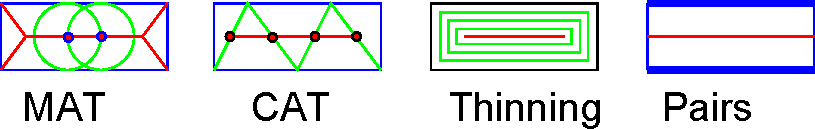
\includegraphics[width=0.6\linewidth]{..//Common/images/MedialMethodsOnlyShort.pdf}
		\caption{Medial Computation Techniques}
		\label{fig:medials}
	\end{figure}



MAT is a locus of the center of an inscribed maximal disc as it rolls around the object's interior.  In 2D, it is called Medial Axis Curve, where as in 3D, it is called Medial Surface. As a formal definition is available, it can be generated for any shape, but the major drawback of this technique is that it creates unnecessary branches and gives unpredictable output due to perturbations on the input shape.

MA involves identifying ``face pairs'', constructing midsurface patches for each and then build a connected midsurface by extend-trim-sewing the patches. This surface-pairing approach has benefits over MAT techniques because the resultant geometry is cleaner and requires lesser post-processing \cite{Lockett2008}. However, as there is no formal definition of this, the surface pairing approach is mostly heuristic in nature. It has difficulty in identification of the surface pairs as well as in joining the midsurface patches. Many of the commercial CAD-CAE packages use this approach and thus, have to provide manual/semi-automatic methods to correct the failures.

Feature-based approaches leverage the use of feature information in the computation of the midsurface.  Information readily available in the feature has been used by few to compute midsurface patches \cite{Robinson2006, DengBrittonLamTorMa2002}, whereas few others work on the final solid shape, recognize features  after decomposition and then create midsurface \cite{Chong2004, Boussuge2013, Boussuge2013a, Woo2013}. The work done so far seems limited to very basic shapes and interactions. There does not seem to be any technique for a variety of features and a generic logic for computing the midsurface.
 
 \subsection{Defeaturing}
 
Defeaturing means removal of unwanted features.  Thakur et al. \cite{Thakur2009} surveyed and classified various techniques used till then, into categories such as surface-based, volume-based and feature-based.  The research presented  here proposes a feature-based defeaturing technique having two approaches, one, specific to sheet metal parts and the other, a generic size-based approach.  Here, defeaturing considered as as purely CAD operation and  calculates a ``gross shape'', which represents the original shape with far lesser details. It does not take into account the usual CAE inputs such as load paths, boundary conditions symmetry, etc. thus making it suitable even for other operations like shape matching, retrieval, etc. CAE inputs can also be integrated on top, as per the requirements. After defeaturing, the model gets simplified and results into the gross shape for which midsurface computation is more effective.
 
Dabke \cite{Dabke1994} through the concept of ``global idealization'', was one of the first researchers to leverage the feature information for defeaturing. His technique was based on heuristic rules derived from the analyst's experience but was rudimentary in the range of usages. Lee \cite{Lee2005, SangHunLee2005, Lee2009} elaborated a technique to reorder features in the history tree and then build partly upto the given level of simplification. Since Brep (Boundary representation) re-evaluation is computationally intensive, he used the cellular model for increasing the performance. One of the major limitations of this approach is that once the model is converted to cellular, its feature update capability would cease to exist, making it difficult for bidirectional change propagation. Russ \cite{Russ2012} mentioned that the determination of the non-critical (suppressible) features relies on the feature type, feature dimensions, proximity of features to the boundary conditions, analysis type, and part dimensions.

	Commercial packages like ACIS\textsuperscript{\textregistered}, Autodesk Fusion\textsuperscript{\textregistered}, Altair's Hypermesh\textsuperscript{\textregistered}, etc. also provide similar defeaturing capabilities mainly for CAE analysis, but are mostly simplistic and size-based in nature.
	
\subsection{Feature Abstraction}
Features, not only carry shape information (geometry and topology) but also embed meta-information based on the application context. With a variety of applications, each having its own need  has resulted into various {\em feature-schemes} not only in different CAD applications, but also in various environments present within the same CAD application.  This causes plethora of cases to deal with for writing a generic algorithm/process. Abstraction alleviates this problem by the extraction of a generic feature-form.  In the context of current research, it means finding of a generic feature, which will represent most of the available features.
 
  Middleditch  provided feature abstraction by proposing structure, construction sequence and point-set, so as to separate issues of  solid modeling, feature modeling and constraints \cite{Middleditch1997}.  Tessier tried to formulate features in terms of generic attributes such reference attributes for reference planes, parameter attributes for model type, depth, etc.\cite{Tessier2013}. 
  
From the research reviewed so far, it appears that there is no feature abstraction generic enough to represent mechanical CAD form features. This research attempts to propose one by  abstracting form features as generic Loft/Sweep feature, with profiles and a guide curve.
  
 \subsection{Cellular Decomposition}
 
Cellular decomposition, in the context of the current research, is the division of a feature-based CAD model into non-volumetrically overlapping, but surface-touching sub-solids.  Research for  cellular decomposition (especially for Computer-aided Manufacturing, and CAE meshing) is going on for decades. Feature-based cellular decomposition, which deals with either decomposition of features, or feature-recognition after decomposition,  has also been  researched extensively \cite{Bidarra1993, BidarraKrakerBronsvoort1998, Woo2003, JaeLee2004, Treeck, Boussuge2013a, Wu2014, Woo2014}. There have been a few attempts to compute a midsurface using cellular-decomposition as well \cite{Chong2004, Woo2013, Boussuge2013, Zhu2015}, but the methodologies presented therein appear limited due to extensive use heuristic rules such as hard-coded values for detecting edge/face pairs, support for limited types of geometries,   limited scope in terms of the range of connections  handled, etc.

Chong et al. \cite{Chong2004} split the solid model into sub-volumes which, in turn, extracted their own midsurface patches. Kageura \cite{Kageura2009} has filed US Patent 2009/0271156 A1 in which a shape is partitioned first, adjacency information is generated and then a midsurface patch is extracted.  Cao \cite{Cao2009} \cite{Cao2011} decomposed the final solid and recognized additive remnant swept primitives, got their sketches, computed midcurves for edge-pairs and created midsurface patches but the joining logic was not much elaborated. Boussuge et al.  \cite{Boussuge2013,Boussuge2013a}  split the solid body at concave edges, recognized (only) positive  protrusion features in the sub-volumes and then idealized each to a midsurface with a joining logic restricted to only a couple of had-coded interaction types. Woo \cite{Woo2013} used his maximal volume technique (\cite{Woo2006, Woo2009} ) and computed midsurface for each sub-volume using face-pair technique. It worked only for analytical surfaces and parallel face pairs

\subsection{Analysis of the Survey findings}
 
 After analyzing various past approaches, both in academic and commercial domains, it can be concluded that,  there has been limited success in the computation of a well-connected midsurface. Many approaches are heavily heuristic, non-generic and need post-processing like, pruning erroneousness branches, extending-trimming to join gaps, removing overlapping surfaces, etc.  By far, the most widely used approach appears to be Midsurface Abstraction (Face Pairing), but even that also is not devoid of issues.  Two of the most critical problems are elaborated below:
	

\begin{itemize}[noitemsep,topsep=2pt,parsep=2pt,partopsep=2pt]%leftmargin=*
	\item  \textbf{Face Pairs Detection Problem}:  \label{sec:facepairdetection}
Face pairs act like a virtual decomposition of a solid into sub-volumes. In MA, each sub-volume computes its own midsurface patch. Finding face-pairs in a complex part is challenging \cite{Boussuge2013}. To address this, feature-information in a feature-based CAD models can be leveraged.  Features are the sub-volumes (called ``canonical'' or ``tool-body'' volumes), created using input feature parameters, which are booleaned at each step in the history tree. Instead of detecting face pairs in the final solid shape, the feature-sub-volumes can be used to compute the midsurface patch.  Here, due to a large number of feature types, writing midsurface-computation for all the feature types separately becomes a tedious task. The solution proposed for this issue is to abstract/generalize these individual features types into some generic form and then compute midsurface patches for just the generic type. Feature abstraction called ``ABEL'' has been proposed to generalize the form features into a generic ``Sweep/Loft'' feature having a profile and a guide curve. Midsurface patch can then be computed by sweeping midcurve of the profile along the guide curve (Section \ref{sec:scell}). %%%%%%%% ADD (\cite{YogeshIITG2014}) LATER

	\item  \textbf{Face-Pair Interaction Problem}: \label{sec:facepairinteraction}
Midsurface patches need to be connected in a similar manner as the face-pairs in the input model are interacted/connected. As there is no theoretical framework encompassing all the possible interaction types, providing a unified logic has not been possible (\cite{Stolt2006}).   Developing a connection logic for each of these types separately can be a tedious task. This research proposes  leveraging of feature-based cellular decomposition to decompose the given solid into sub-volumes and then devise a generic logic for joining the midsurface patches (Section \ref{sec:icell}).
\end{itemize}
 